\section{Casi d'uso}
I casi d'uso seguenti emergono da un'attenta analisi degli \textit{Analisti} del gruppo \GroupName{} rivolta al capitolato e da un'approfondita discussione con il proponente \Proponente{}. Gran parte dei casi d'uso sono stati dedotti grazie all'esperienza derivata dall'utilizzo di \glossario{ActiveAdmin}, un progetto analogo a \ProjectName{} basato su \glossario{Ruby on Rails}.\\
Ogni caso d'uso è identificato univocamente e in modo gerarchico tramite una codifica nella forma:
\begin{center}
	\textit{UC[codice dell'ambito][codice univoco del padre],[codice progressivo del figlio]}
\end{center} 
dove il \textbf{codice dell'ambito} può assumere i seguenti valori:

\begin{itemize}
	\item \textbf{U} - ambito utente, che comprende sia l'utente normale che l'\textit{admin} di una applicazione generata da \ProjectName{};
	\item \textbf{S} - ambito sviluppatore.
\end{itemize}


\subsection{Ambito Utente}
	\subsubsection{UCU: Operazioni ad alto livello}
		
		\begin{figure}[H]
    		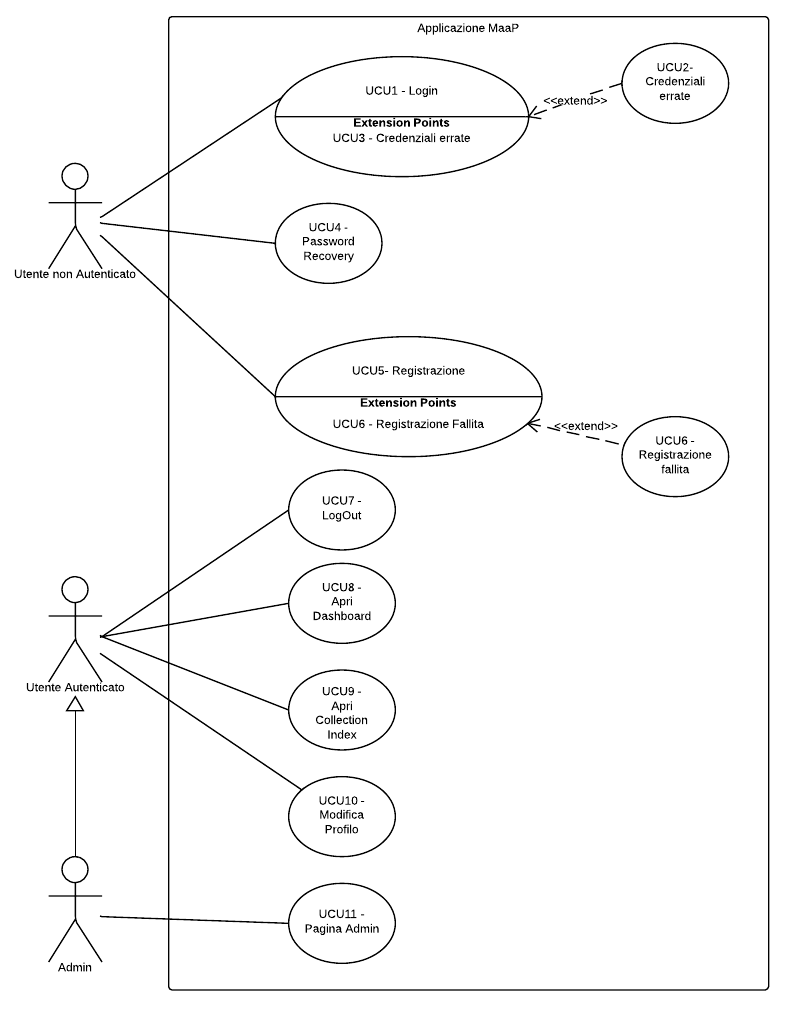
\includegraphics[width=12cm]{UML/UCU - Operazioni ad alto livello.png}{\centering}
    		\caption{UCU - Operazioni ad alto livello}
		\end{figure}
			
		%Tabella 
		\begin{table}[H]
		\begin{longtabu}{  c | X  }
						
		\hline
		\multicolumn{2}{ | c | }{ \cellcolor[gray]{0.9} \textbf{UCU: Operazioni ad alto livello} } \\ 
		\hline
			
			\textbf{Attori Primari} & 
			Utente non autenticato, Utente autenticato, Admin \\
    			
    		\textbf{Attori Secondari} &  \\
    			
    		\textbf{Scopo e Descrizione} & 
    		L'Utente non autenticato può autenticarsi inserendo le credenziali nell'apposito form e recuperare le stesse qualora le abbia perse. L'Utente autenticato in qualsiasi punto dell'applicazione può accedere alle seguenti funzionalità: accedere alla Dashboard, effettuare il Logout , può scegliere una qualsiasi collection presente e può modificare i propri dati. L'Utente Admin eredita le funzionalità dell'Utente Autenticato ed in più accedere alla sezione "Admin" nella quale può creare o modificare un nuovo utente.\\ 
    			
    		\textbf{Precondizioni}  & 
    		L'applicazione Maap è funzionante e pronta all'utilizzo. \\ 
    			
    		\textbf{Postcondizioni} &
    		L'applicazione ha ricevuto le informazioni sulle operazioni che l'utente vuole eseguire. \\
    			
    		\textbf{Flusso Principale} & 
			1. Utente non autenticato esegue il login (UCU1); 2. Utente non autenticato può recuperare la password (UCU4); 3. Utente non autenticato può richiedere la registrazione (UCU5); 4. L'utente autenticato può decidere di effettuare il logout (UCU7); 5. L'utente autenticato può visualizzare la Dashboard (UCU8); 6. L'utente autenticato può scegliere una collection e visualizzarla (UCU9); 7. L'utente autenticato può scegliere di modificare i propri dati (UCU10); 8. L'admin può accede alla sua pagina di amministrazione (UCU11). \\
    				
    		\textbf{Scenari Alternativi} & . \\
  
  		\end{longtabu}
		\end{table}
\clearpage

